In this section, we start with the explanation of the proposed model's establishment where the necessary parameters including $\{\alpha_{P}, \alpha_{R}, \alpha_{RP}\}$, ${\{\beta_{1}, \beta_{2}, \beta_{3}\}}$ and $\{\lambda_{1}, \lambda_{2} \}$ are numerically determined. Afterward, we briefly evaluate and discuss the prediction performance of our model. The evaluation is two-fold. First, the prediction performance of the proposed model is quantitatively and qualitatively assessed on test videos in a specific database \cite{LFOVIA}. Second, a subjective test is conducted in order to evaluate how well the predicted cumulative QoE correlates with subjective cumulative evaluation at different moments of a streaming session. Finally, the complexity of the proposed model is also analyzed for real-time cumulative QoE prediction.


%/===============================
\subsection{Model Establishment}
\label{section:Training}

  The parameters of the proposed model was computed according to a four-step procedure as follows: 
 
  \begin{enumerate}[label=\arabic*)]
    \item A specific publicly available database was employed for establishing and evaluating the proposed model. 
    \item An LSTM-QoE model \cite{QoEModel_LSTM} was trained to predict the instantaneous QoE values.
    \item The memory effects' parameters $\{ \alpha_{P}, \alpha_{R}, \alpha_{RP} \}$ were computed to form the memory weight vector.
    \item The coefficients of memory weight ${\{\beta_{1}, \beta_{2}, \beta_{3}\}}$ in Eq. \ref{eqn:Weight} and the parameters of the proposed model $\{ \lambda_{1}, \lambda_{2} \}$ in Eq. \ref{eqn:Cumulative_QoE} were determined through the predicted instantaneous QoE values and the subjective DoI collected from the experiment in subsection 3.3.
  \end{enumerate}
  The details of each step are described in the next sub-subsections.
  
  
  \subsubsection{Database description} \label{section:DatabaseDescription}
    Our model was established and evaluated based on a set of 36 distorted videos in LFOVIA Video QoE Database \cite{LFOVIA}. These videos have different playout patterns distorted by bitrate switching and rebuffering events. In this database, the overall QoE and the time-varying instantaneous QoE scores for those videos were obtained are in the range [0, 100], with score 0 being the worst and 100 being the best. The set of distorted videos was divided into training and testing sets with a training:testing ratio of 80:20. Accordingly, there were 28 videos in the training set and 8 videos in the testing set. The training and testing set were respectively used to obtain the model parameters described in sub-subsection \ref{parameter} and evaluate the prediction performance of the model presented in subsection \ref{section:ObjectiveEvaluation}.

  \subsubsection{Instantaneous QoE Prediction by LSTM-QoE}
  The instantaneous QoE values were estimated by the LSTM-QoE model \cite{QoEModel_LSTM}. The model was trained on the training set with 28 distorted videos driven by 4 features $STSQ$, $PI$, $NR$ and $TR$. The performance of this model was then quantified on the 8 test videos using the Pearson Correlation Coefficient (PCC) and Spearman Rank Order Correlation Coefficient (SROCC). Consequently, the model achieved high accuracy with PCC of \textbf{0.9946} and SROCC of \textbf{0.8870}. The performance of the trained model is illustrated in Figure \ref{fig:LSTM_Performance}, demonstrating high accurate prediction. 

\begin{figure}[tb]
  \centering
  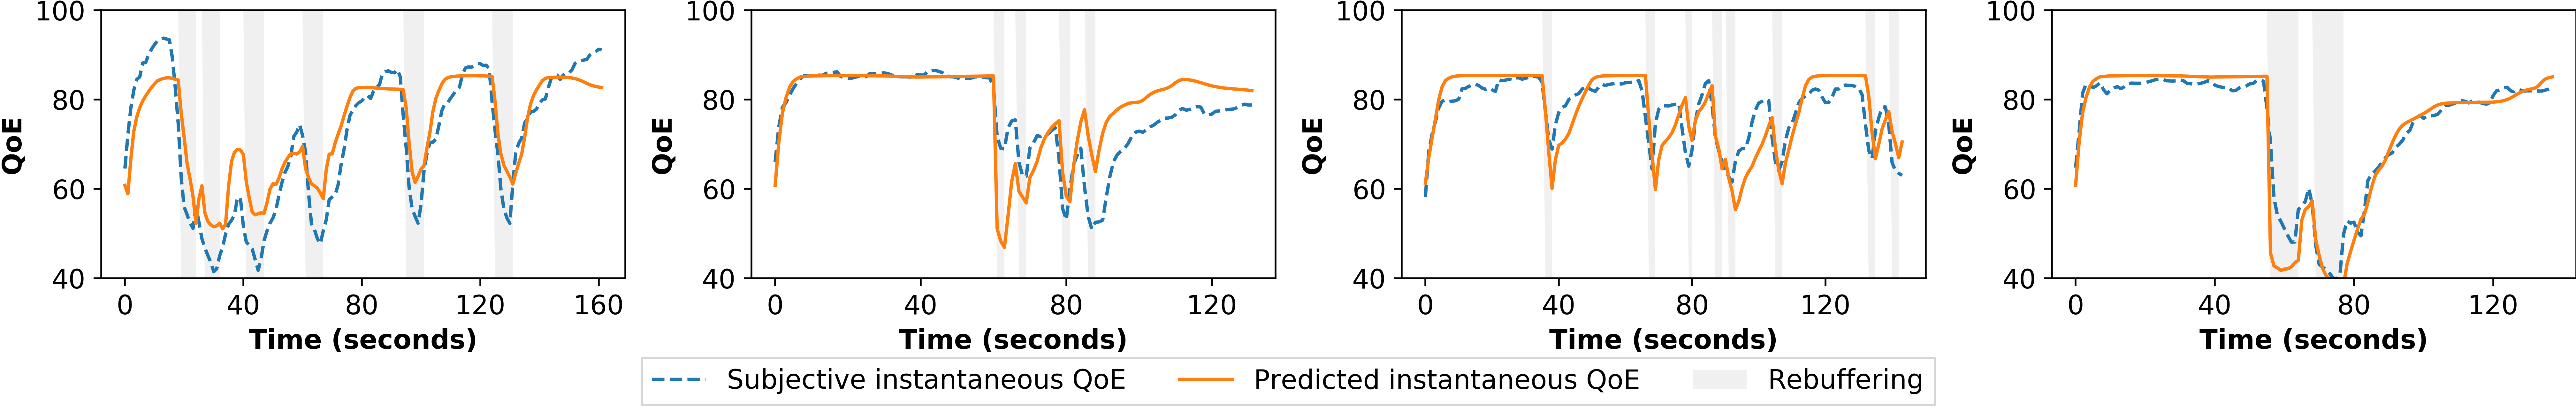
\includegraphics[width=\linewidth]{\FigsDir/lstm_accuracy.png}
  \caption{Some examples of instantaneous QoE prediction performance obtained from the LSTM-QoE model on different test videos of the database.}
  \label{fig:LSTM_Performance}
\end{figure}

  \subsubsection{Parameters Selection}
  \label{parameter}
  As discussed in subsection~\ref{section:MemoryEffects}, the parameters $\{ \alpha_{P}, \alpha_{R}, \alpha_{RP} \}$ indicate how memory factors impact the perceived video quality over time. The larger $\{\alpha_{P}, \alpha_{R}, \alpha_{RP} \}$ are, the easier it is for the user to forget. According to \cite{PrimacyVsRecency, NetflixQoE}, the effects of primacy and recency gradually decrease within 15 to 20 seconds. Therefore, the deteriorating time was set to 15 seconds. Since the user usually recalls unpleasant events when providing a QoE score, the effect of repetition is larger and remain longer than primacy and recency. As a result, the values of $\alpha_{RP}$ must be smaller than $\alpha_{P}$ and $\alpha_{R}$. The effect of repetition will remain within 30 seconds. The function $solve$ in MATLAB \cite{MATLAB} was employed to compute the parameters $\alpha_{P}$, $\alpha_{R}$, and $\alpha_{RP}$ according to Eq.~\ref{eqn:Primacy}, \ref{eqn:Recency}, and \ref{eqn:Repetition}, respectively. Consequently, the obtained values of parameters $\{ \alpha_{P},\alpha_{R}, \alpha_{RP} \}$ are shown in Table \ref{tbl:Parameters_MemoryEffects}.
  
\begin{table}[tb]
  \caption{Parameters of the primacy and recency effect, forgetting curve and repetition}
  \centering
  \begin{tabular}{|ccc|}
    \hline
    $\bm{\alpha_{P}}$ & $\bm{\alpha_{R}}$ & $\bm{\alpha_{RP}}$\\
    \hline
    0.6807 & 0.6807 & 0.3404\\
    \hline
  \end{tabular}
  \label{tbl:Parameters_MemoryEffects}
\end{table}


\begin{table}[tb]
  \caption{Parameters of memory weight and the cumulative QoE model}
  \centering
  \begin{tabular}{|ccc|cc|}
    \hline
    $\bm{\beta_{1}}$ & $\bm{\beta_{2}}$ & $\bm{\beta_{3}}$ & $\bm{\lambda_{1}}$ & $\bm{\lambda_{2}}$\\
    \hline
    0.0284 & 0.8492 & 0.1177 & 0.9809 & 0.0800\\
    \hline
  \end{tabular}
  \label{tbl:Parameters_CumulativeQoE}
\end{table}


Thereby, the parameters $\{\beta_{1}, \beta_{2}, \beta_{3}\}$ and $\{ \lambda_{1}, \lambda_{2} \}$ of weight memory and the proposed cumulative QoE model are now can be estimated. Considering a streaming session with a video in the training set of $L$ seconds, the cumulative QoE from the beginning to the end of the streaming session was calculated as follows:
  
\begin{equation}
\begin{split}
  CQ_{L} &= \lambda_{1} \left ( {Q}_{L}\times{W}^{T}_{L} \right ) + \lambda_{2}DoI \\
         &= \lambda_{1} \sum_{i=0}^{L}{w_{i}q_{i}} + \lambda_{2}DoI \\
         &= \lambda_{1} \sum_{i=0}^{L}{\left ( \beta_{1}f_{P}(i) + \beta_{2}f_{R}(i) + \beta_{3}f_{RP}(i) \right ) q_{i}} + \lambda_{2}DoI
\end{split}
\end{equation}
where, ${Q}_{L}$ is the vector of instantaneous QoE $(q_{0},  q_{1}, \dots, q_{L})$,  ${W}_{L}$ is the memory weight vector $(w_{0},  w_{1}, \dots, w_{L})$.


As mentioned in subsection \ref{section:CumulativeQoE}, the cumulative QoE at the end of the session $CQ_{L}$ is also considered as the overall QoE. Therefore, we first need to minimize the least square error:

\begin{equation}
    \bm{J} = \left \| CQ_{L} - Q_{overall} \right \|^{2}
\end{equation}


where $Q_{overall}$ is the subjective overall user's QoE obtained from the database. A curve fitting is performed using \textit{lsqcurvefit} in MATLAB \cite{MATLAB} with 28 training videos to obtain the memory weight parameters $\{\beta_{1}, \beta_{2}, \beta_{3}\}$ and the cumulative QoE parameters $\{ \lambda_{1}, \lambda_{2} \}$. The numerical values of those parameters are shown in Table~\ref{tbl:Parameters_CumulativeQoE}.


% \revise{We found that $\lambda_{1}$ is highest, which is about 5 times higher than $\lambda_{2}$ and $\lambda_{3}$. According to Eq. \ref{eqn:Cumulative_QoE}, this shows that the impact of the past experience is strongest, and the impact of the DoI is lowest.}
    


%/=================================================
\subsection{Performance Evaluation on Testing Videos}
\label{section:ObjectiveEvaluation}
  
  After obtaining the necessary parameters for the proposed model, we quantitatively and qualitatively evaluate its prediction performance on 8 distorted videos in the testing set. Alternatively, the discussion on the results is also performed.

To quantitatively assess the prediction performance, the correlation between the subjective overall QoE obtained in the LFOVIA Video QoE Database \cite{LFOVIA} and our predicted cumulative QoE at the end of each video was computed. It is crucial to note that the subjective overall QoE can be considered as the cumulative perception of the user at the end of streaming session. There were three evaluation metrics utilized for evaluation: 1) Pearson Correlation Coefficient (PCC), 2) Spearman Rank Order Correlation Coefficient (SROCC), and 3) Root Mean Square Error (RMSE). Typically, PCC and SROCC quantify how well the predicted QoE tracks the actual QoE scores in the database, whereas, RMSE indicates the closeness between them. We also compared our proposed model with a reference method of \cite{CumulativeQoE_Assessing}, using the same training set and testing set. The cumulative QoE model in \cite{CumulativeQoE_Assessing} is characterized by the following equation: 

\begin{equation}
    Q_{t} = \gamma Q_{t-1} + (1-\gamma)q_{t}
\end{equation}

where $q_{t}$ is the instantaneous user experience at moment $t$, $Q_{t-1}$ is the cumulative QoE at the previous moment $t-1$, and $\gamma$ is the memory strength parameter. The correlation between the predicted cumulative QoE obtained from this model and the subjective overall QoE in LFOVIA database was also investigated through PCC, SROCC and RMSE metrics. We reported the performance of our model and the reference method in Table \ref{tbl:PerformanceDataset}. This result shows a superior prediction performance of our model. Figure \ref{fig:PCC_CumulativeQoe_OverallQoE} additionally emphasizes the competitive performance of our model. Thereby, the proposed model has effectively assessed cumulative perception over multiple scenarios in testing videos. 

% \begin{table}[tb]
%   
%   \centering
%   \begin{tabular}{cccc}
%     \toprule
%     & $\textbf{PCC}$ & $\textbf{SROCC}$ & $\textbf{RMSE}$\\
%     \midrule
%     \cite{CumulativeQoE_Assessing} & 0.4292 & 0.4048 & 7.931 \\
%     Proposed Model & \textbf{0.7664} & \textbf{0.7857} & \textbf{4.654} \\
%     \bottomrule
%   \end{tabular}
%   \label{tbl:PerformanceDataset}
% \end{table}

\begin{table}[tb]
\caption{Prediction performance of the reference model and our proposed model over training and testing set}
\centering
\begin{tabular}{|l|l|c|c|c|}
\hline
& & PCC & SROCC & RMSE \\
\hline
\multicolumn{1}{|l|}{\multirow{2}{*}{Training}}   & \multicolumn{1}{l|}{\cite{CumulativeQoE_Assessing}}                  & 0.7413       & 0.6420         & 10.6187        \\
\multicolumn{1}{|l|}{}                                & \multicolumn{1}{l|}{Proposed model}  & \textbf{0.9441}       & \textbf{0.8604}         & \textbf{4.1525}         \\
\hline
\multicolumn{1}{|l|}{\multirow{2}{*}{Testing}}    & \multicolumn{1}{l|}{\cite{CumulativeQoE_Assessing}}                  & 0.2777       & 0.2381         & 7.5135         \\
\multicolumn{1}{|l|}{}                                & \multicolumn{1}{l|}{Proposed model}  & \textbf{0.7664}       & \textbf{0.7857}         & \textbf{4.6538}         \\
\hline
\end{tabular} \label{tbl:PerformanceDataset}
\end{table}


\begin{figure}[tb]
  \centering
  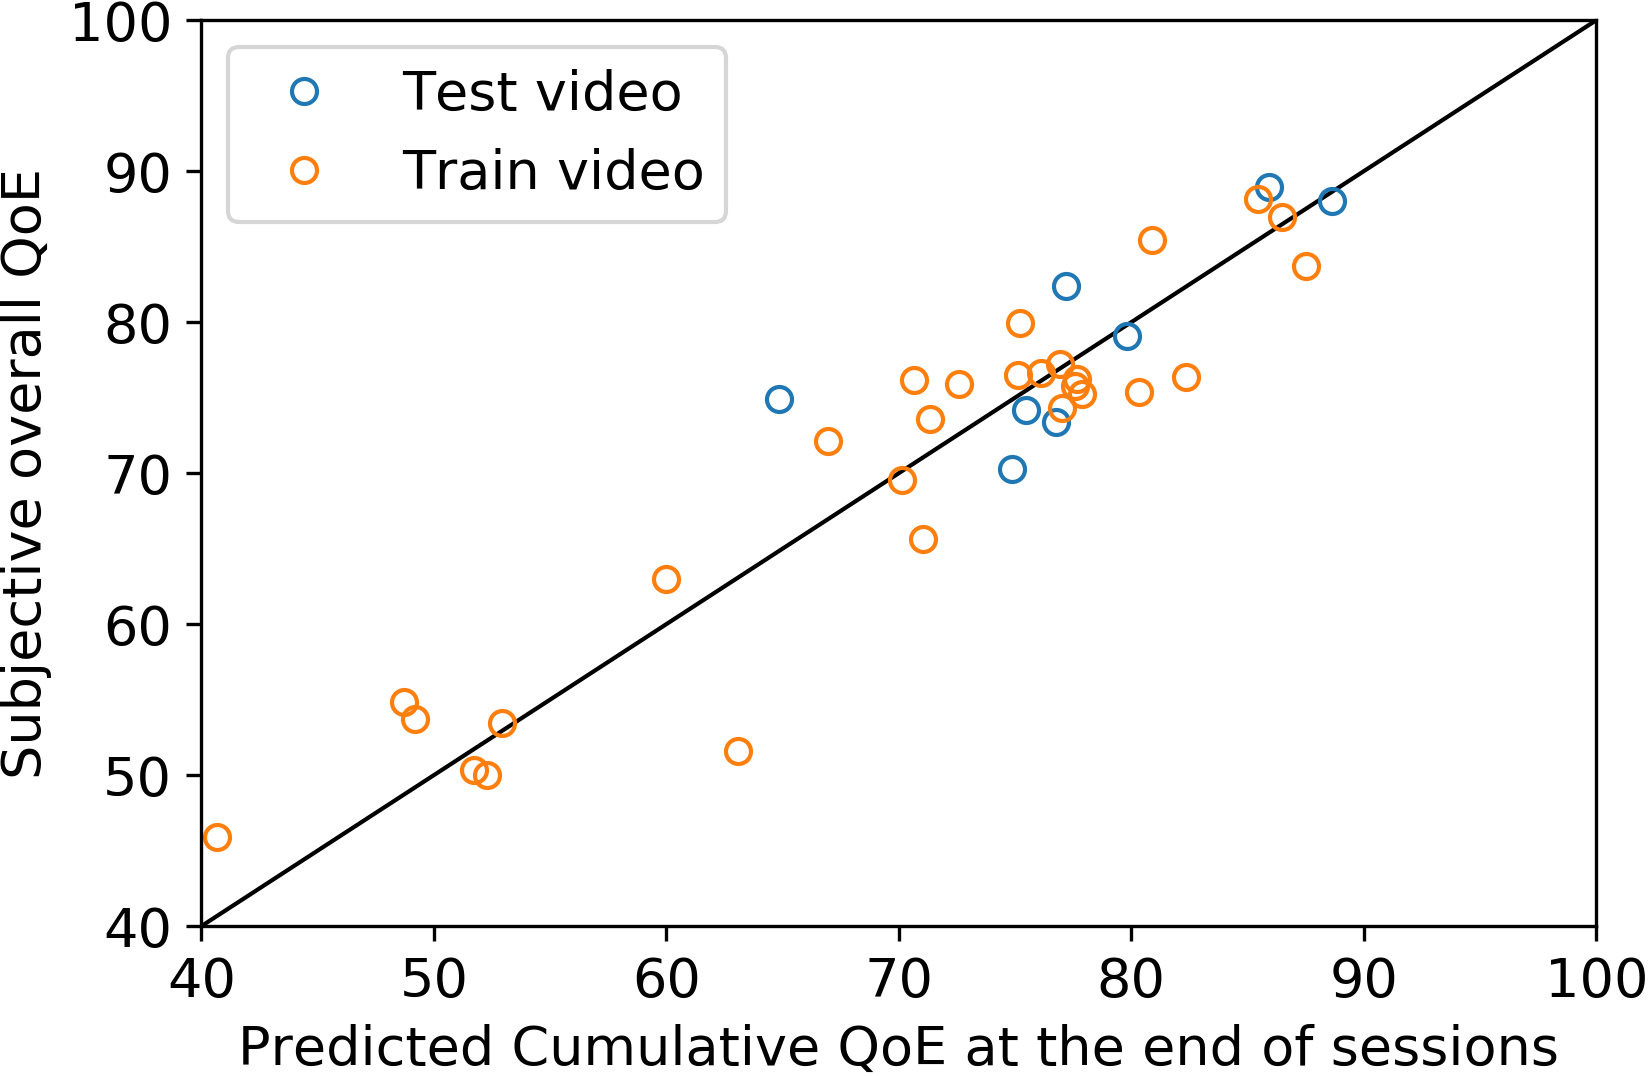
\includegraphics[width=0.5\linewidth]{\FigsDir/pcc_cmqoe_overallqoe.png}
  \caption{Correlation between subjective overall QoE and predicted cumulative QoE at the end of streaming session}
  \label{fig:PCC_CumulativeQoe_OverallQoE}
\end{figure}

\begin{figure}[tb]
  \centering
  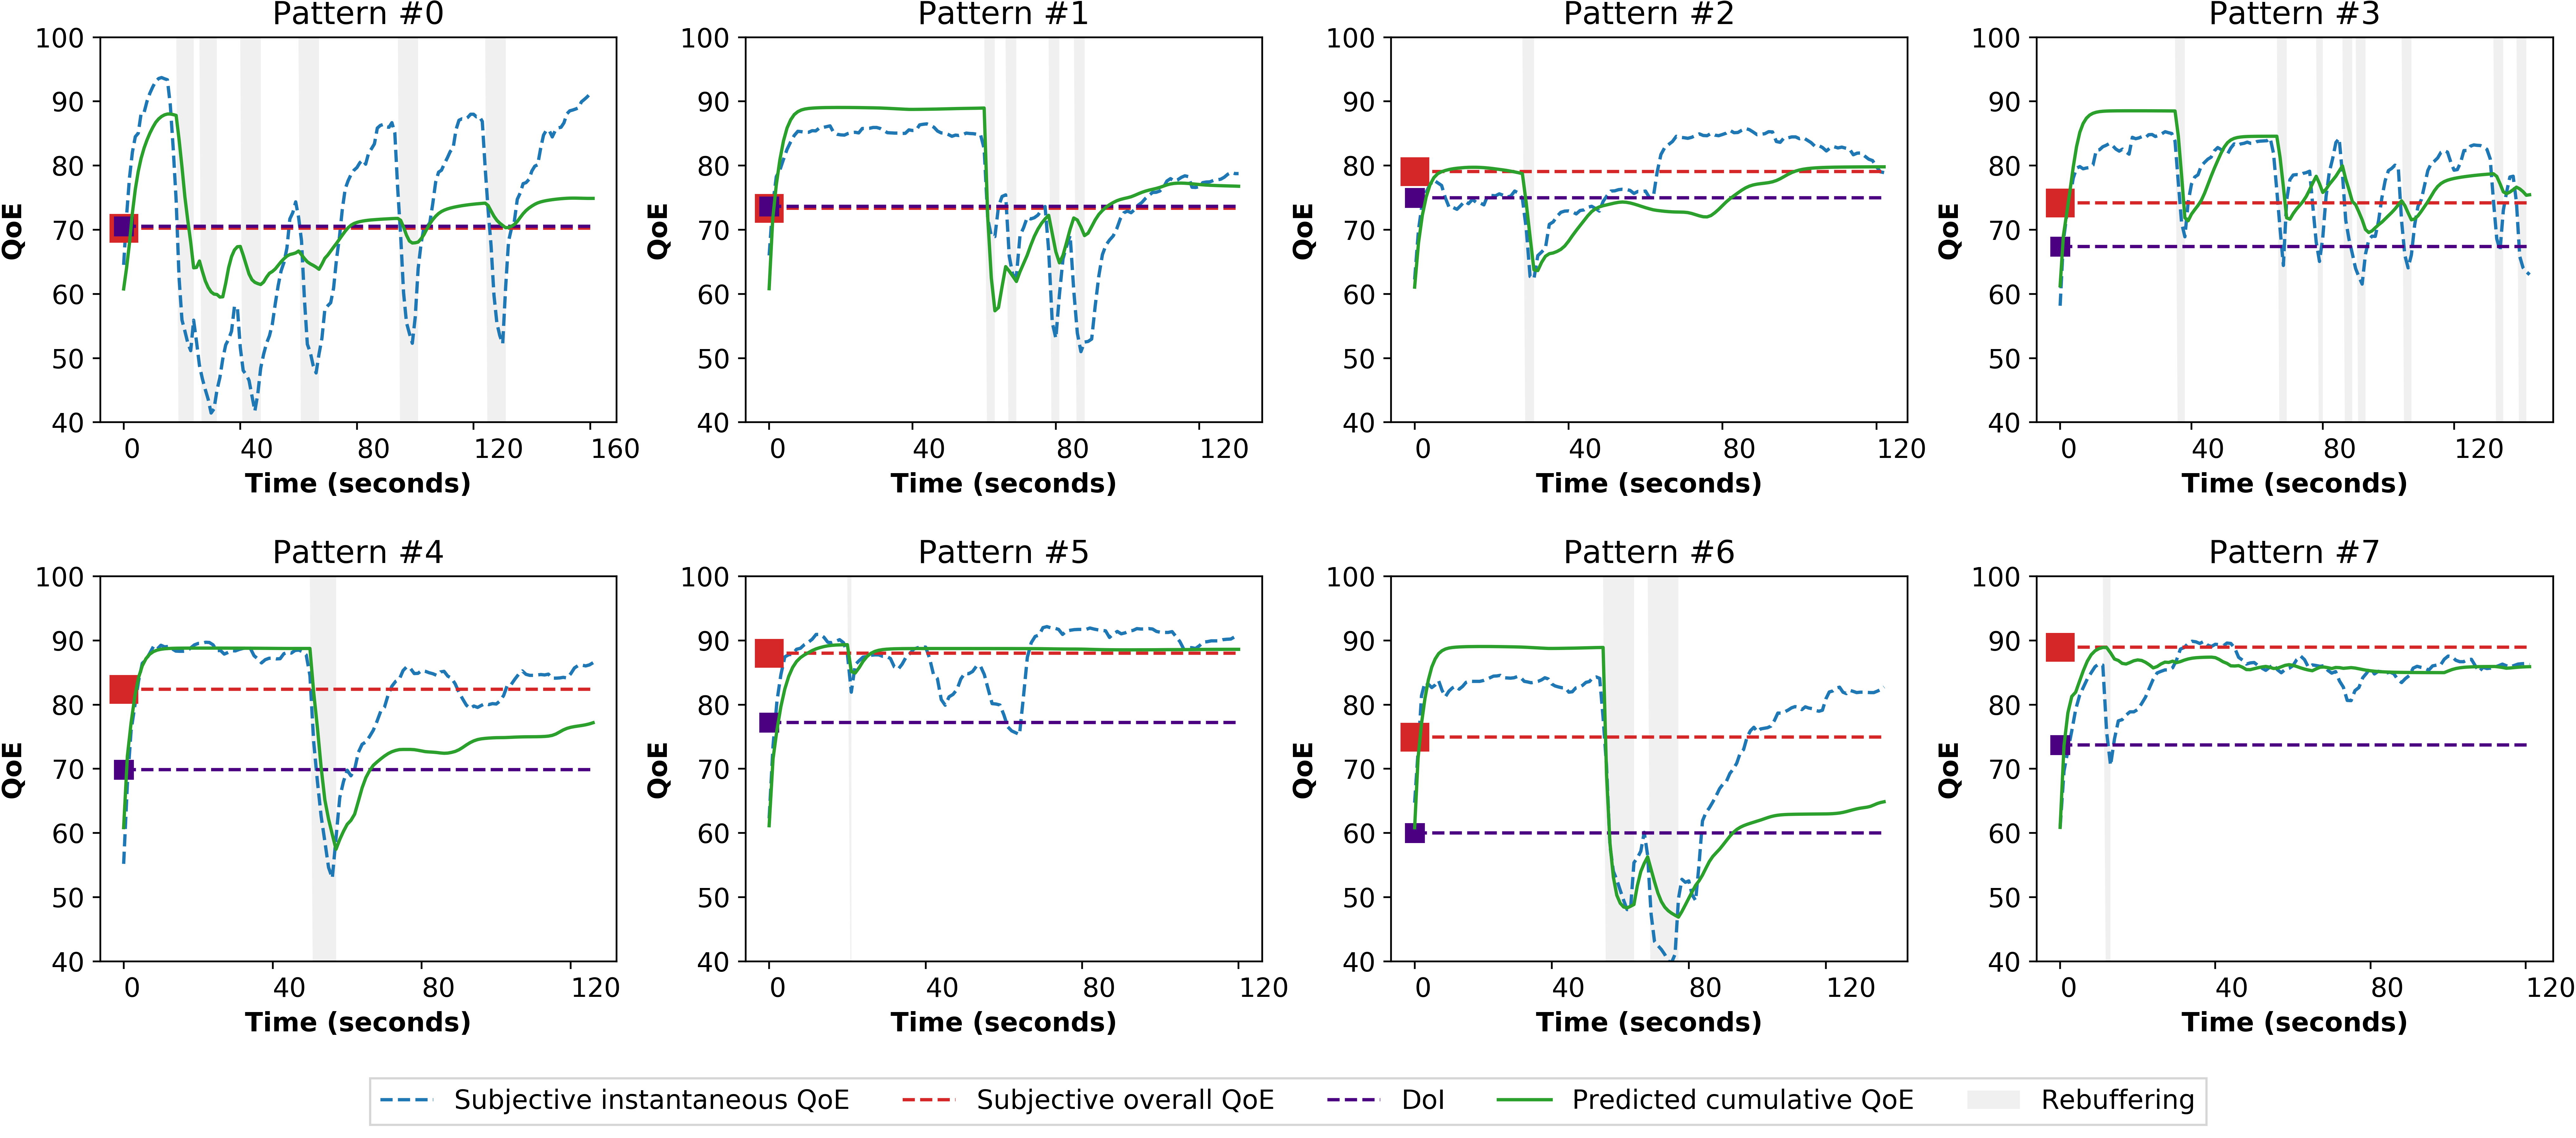
\includegraphics[width=\linewidth]{\FigsDir/cumulative_performance_dataset.png}
  \caption{Predicted cumulative QoE in comparison with the subjective overall and instantaneous QoE over eight different playout patterns}
  \label{fig:Cumulative_Performance}
\end{figure}


In qualitative evaluation, our purpose is to validate the impact of memory effects and DoI on the cumulative QoE prediction over multiple scenarios on testing videos. Thereby, the prediction performance of the proposed model in a short period and longer period can be assessed. For that reason, in Figure \ref{fig:Cumulative_Performance}, we plot the predicted cumulative QoE in comparison with both subjective instantaneous QoE and subjective overall QoE which are obtained from the database. From now, the terms of subjective instantaneous QoE and subjective overall QoE will be referred to as instantaneous QoE and overall QoE for short. 

In general, the predicted cumulative QoE precisely reacts to any interruption at any moment while being close to the overall QoE at the end of the streaming session. For the initial interruption, it is always witnessed a significant deterioration in predicted cumulative QoE. Nevertheless, when such unpleasant events continuously occur, the predicted cumulative QoE tends to decrease at a lower rate. Additionally, a lower recovering rate is subsequently introduced after each event. 

%/=======================================
\subsubsection{Impacts of memory effects}

  In pattern \#2, \#5, \#7, there is only one interruption with short duration occurring near the beginning of streaming sessions. As a result, the predicted cumulative QoE introduces a slight decrease, following by a gradual recovery and convergences at the values as close to the overall QoE. These trends are consistent with those of instantaneous QoE. It means that the prediction accurately demonstrates the role of forgetting curve characteristic as well as the recency effect. More concretely, after the finishing of the interruption, the memory intensity about such event starts to exponentially decay, leading to the recovery in perceived video quality. At the end of streaming sessions, there is a possibility that the decay has completely finished, in other words, the memory of distorted events is vanished. Therefore, the recency effect becomes dominant, leading to the consistency among the predicted cumulative QoE, instantaneous QoE, and overall QoE.
  
  In pattern \#0 and \#1, rebuffering event repeatedly occurs in the middle of streaming sessions. While the predicted cumulative QoE is consistent with the overall QoE at the end of sessions, the instantaneous QoE tends to continuously increase, creating a big gap to the overall QoE. At first sight, one might think that the overall QoE must be as high as the instantaneous QoE at the end of streaming sessions due to the recency effect. This inference is understandable because the moment at which the last interruption occurs is quite far from the end of sessions, thus, the recency effect would have become dominant, resulting in the consistency among those QoE evaluations. However, when the interruption repeats many times, the impact of repetition characteristic become significantly obvious. Consequently, the user tends to provide an overall evaluation whose value is lower than the instantaneous QoE. On the other hand, by considering the recency effect and repetition characteristic, our proposed model can effectively provide the prediction consistency with the overall QoE.
  
  According to the hysteresis effect \cite{TemporalHysteresisModel}, the user is highly sensitive to a single unpleasant event and provides poor QoE scores immediately. However, when the interruption occurs many times as in pattern \#0, \#1 and \#3, the impact of the hysteresis effect will be shared with the repetition characteristic. This makes the user behaves in the consideration of past annoying events to avoid the aggressive reaction. In addition, under the impact of repetition characteristic, such the events are stuck in the user's memory and are recalled when the user provides the overall assessment. However, the instantaneous QoE always aggressively reacts to the distorted events, by dramatically decreasing and quickly recovering during a short period. This is because the instantaneous QoE is estimated locally without considering the global views of the streaming session. Oppositely, by weighting the instantaneous QoE by the memory effects (especially repetition characteristic), the predicted cumulative QoE can react calmly, and, eventually, correlates perfectly with the overall QoE. 
  
  Interestingly, the predicted cumulative QoE also indicates a special behavior in human perception which cannot be found in the instantaneous QoE and overall QoE. We call such the behavior as the \textit{persistent evaluation} where the user seems to familiar with the distorted event and to accept it. The user does not even want to deteriorate their evaluation score or to quit from the streaming session. For instance, pattern \#0 and \#3 visualizes that the cumulative QoE dramatically falls after the occurrence of the first rebuffering event. However, it decreases with a significantly lower amplitude on the ones happening subsequently.

%/============================
\subsubsection{Impacts of DoI}
  As we mentioned in subsection \ref{section:DoI}, the correlation between DoI and subjective overall QoE is modest. However, the contribution of DoI on prediction performance is well recognized in some cases as shown in pattern \#2, \#3, \#5 and \#7 which share a common characteristic where the predicted cumulative QoE correctly meets the overall QoE. To be honest, without DoI ($\lambda_{2}=0$), the predicted cumulative QoE would have been much lower than the overall QoE. Especially, in each pattern \#5 and \#7 where contains only one super-short rebuffering event near the beginning of streaming sessions, the memory intensity about this event must be completely vanished, followed by the dominance of the recency effect, resulting in very high overall QoE. However, the contents of these two videos might not sufficiently interesting to the users, leading to the deterioration in their evaluation. Therefore, when the contribution of DoI is precisely recognized, our proposed model provides an extremely high accurate prediction. However, in pattern \#4 and \#6, there exists long duration interruptions in the middle of streaming sessions, creating significantly high intensity memory about those events. As a result, the predicted cumulative QoE dramatically decreases and slowly recovers. However, the insufficiently accurate contribution of DoI has curbed the recovering rate. Consequently, the predicted cumulative QoE cannot catch up with the overall QoE at the end of streaming sessions. This emphasizes the lack of generalization in DoI coefficient $\lambda_{2}$. We believe that the original reason is the insufficient number of participated subjects in the subjective evaluation in subsection \ref{section:DoI} where each video was watched and evaluated by only 10 subjects. In the future, a larger number of participants must be involved in this experiment. 
  
  %DoI's contribution is not clear compared to the memory effects due to the small value of parameter $\lambda_{2}$. However, in pattern \#4, \#5, \#6 and \#7, it is easy to see that there are a big gap between DoI and the subjective overall QoE.In pattern \#5 and \#7, when a small rebuffering event happens, the predicted cumulative QoE slightly decrease and quickly recover to the same level. However, in pattern \#4 and \#6, the predicted cumulative drastically decrease after the first rebuffering occurrence, and persistently stay at average level while the instantaneous recovers to very high level and being close to the overall QoE. It can be explained by the weighted DoI added into the cumulative QoE is small, resulting small improvement.
  
  %This is because our proposed model takes into consider the low value of DoI resulting a depressed correlation between the overall QoE and the predicted cumulative QoE at the end of sessions. We speculate this as the low correlation between the subjective overall QoE and the DoI obtained from the experiment in subsection \ref{section:DoI}. We believe that the original reason is the insufficient number of participated subjects. In fact, each video in our experiment was watched and evaluated by only 10 subjects. In the future, a larger number of participants must be involved in this experiment.
   
  %at the end of the streaming session correlate slightly worse with the overall QoE compared to that of the instantaneous subjective QoE.  determined by the parameter $\lambda_{2}$. 
  
  %DoI's contribution is not actually clear in this evaluation.
  
%   However, its influence on QoE prediction was not as apparent as we expected. 

%/================================
\subsection{Subjective Evaluation}
\label{section:SubjectiveEvaluation}

  \graphicspath{{Chapter3/Section3.3/Figs/}}


\begin{table}[tb]
  \caption{Prediction performance of reference model and the proposed model over subjective experiment}
  \centering
  \begin{tabular}{|c|c|c|c|c|}
    \hline
    & PCC & SROCC & RMSE & OR (\%)\\
    \hline
    \cite{CumulativeQoE_Assessing} & \textbf{0.5418} & 0.3917 & 9.1318 & 33.3\\ \hline
    Proposed model & 0.5405 & \textbf{0.5146} & \textbf{9.0922} & \textbf{25.0}\\
    \hline
  \end{tabular}
  \label{tbl:PerformanceExperiment}
\end{table}


\begin{figure}[tb]
  \centering
  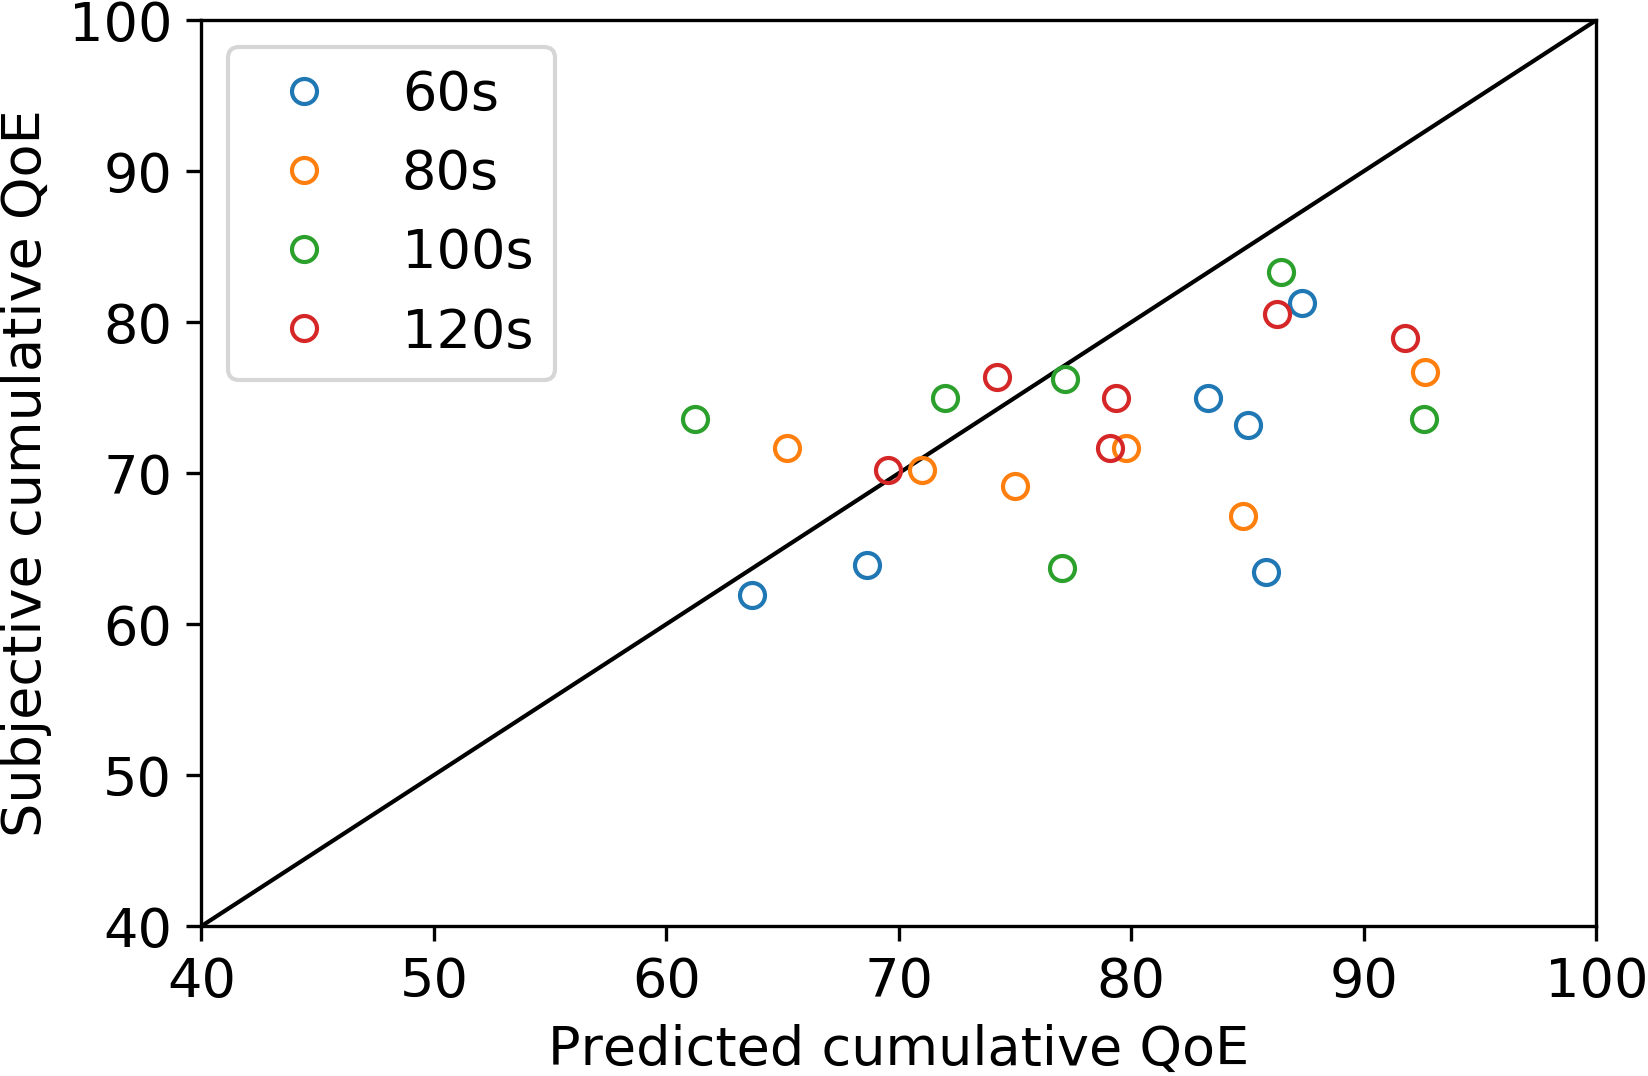
\includegraphics[width=0.5\linewidth]{\FigsDir/pcc_cmqoe_mosqoe.png}
  \caption{Scatter plot of predicted cumulative QoE and subjective cumulative QoE.}
  \label{fig:PCC_CumulativeQoE_MOSQoE}
\end{figure}

\begin{figure}[tb]
  \centering
  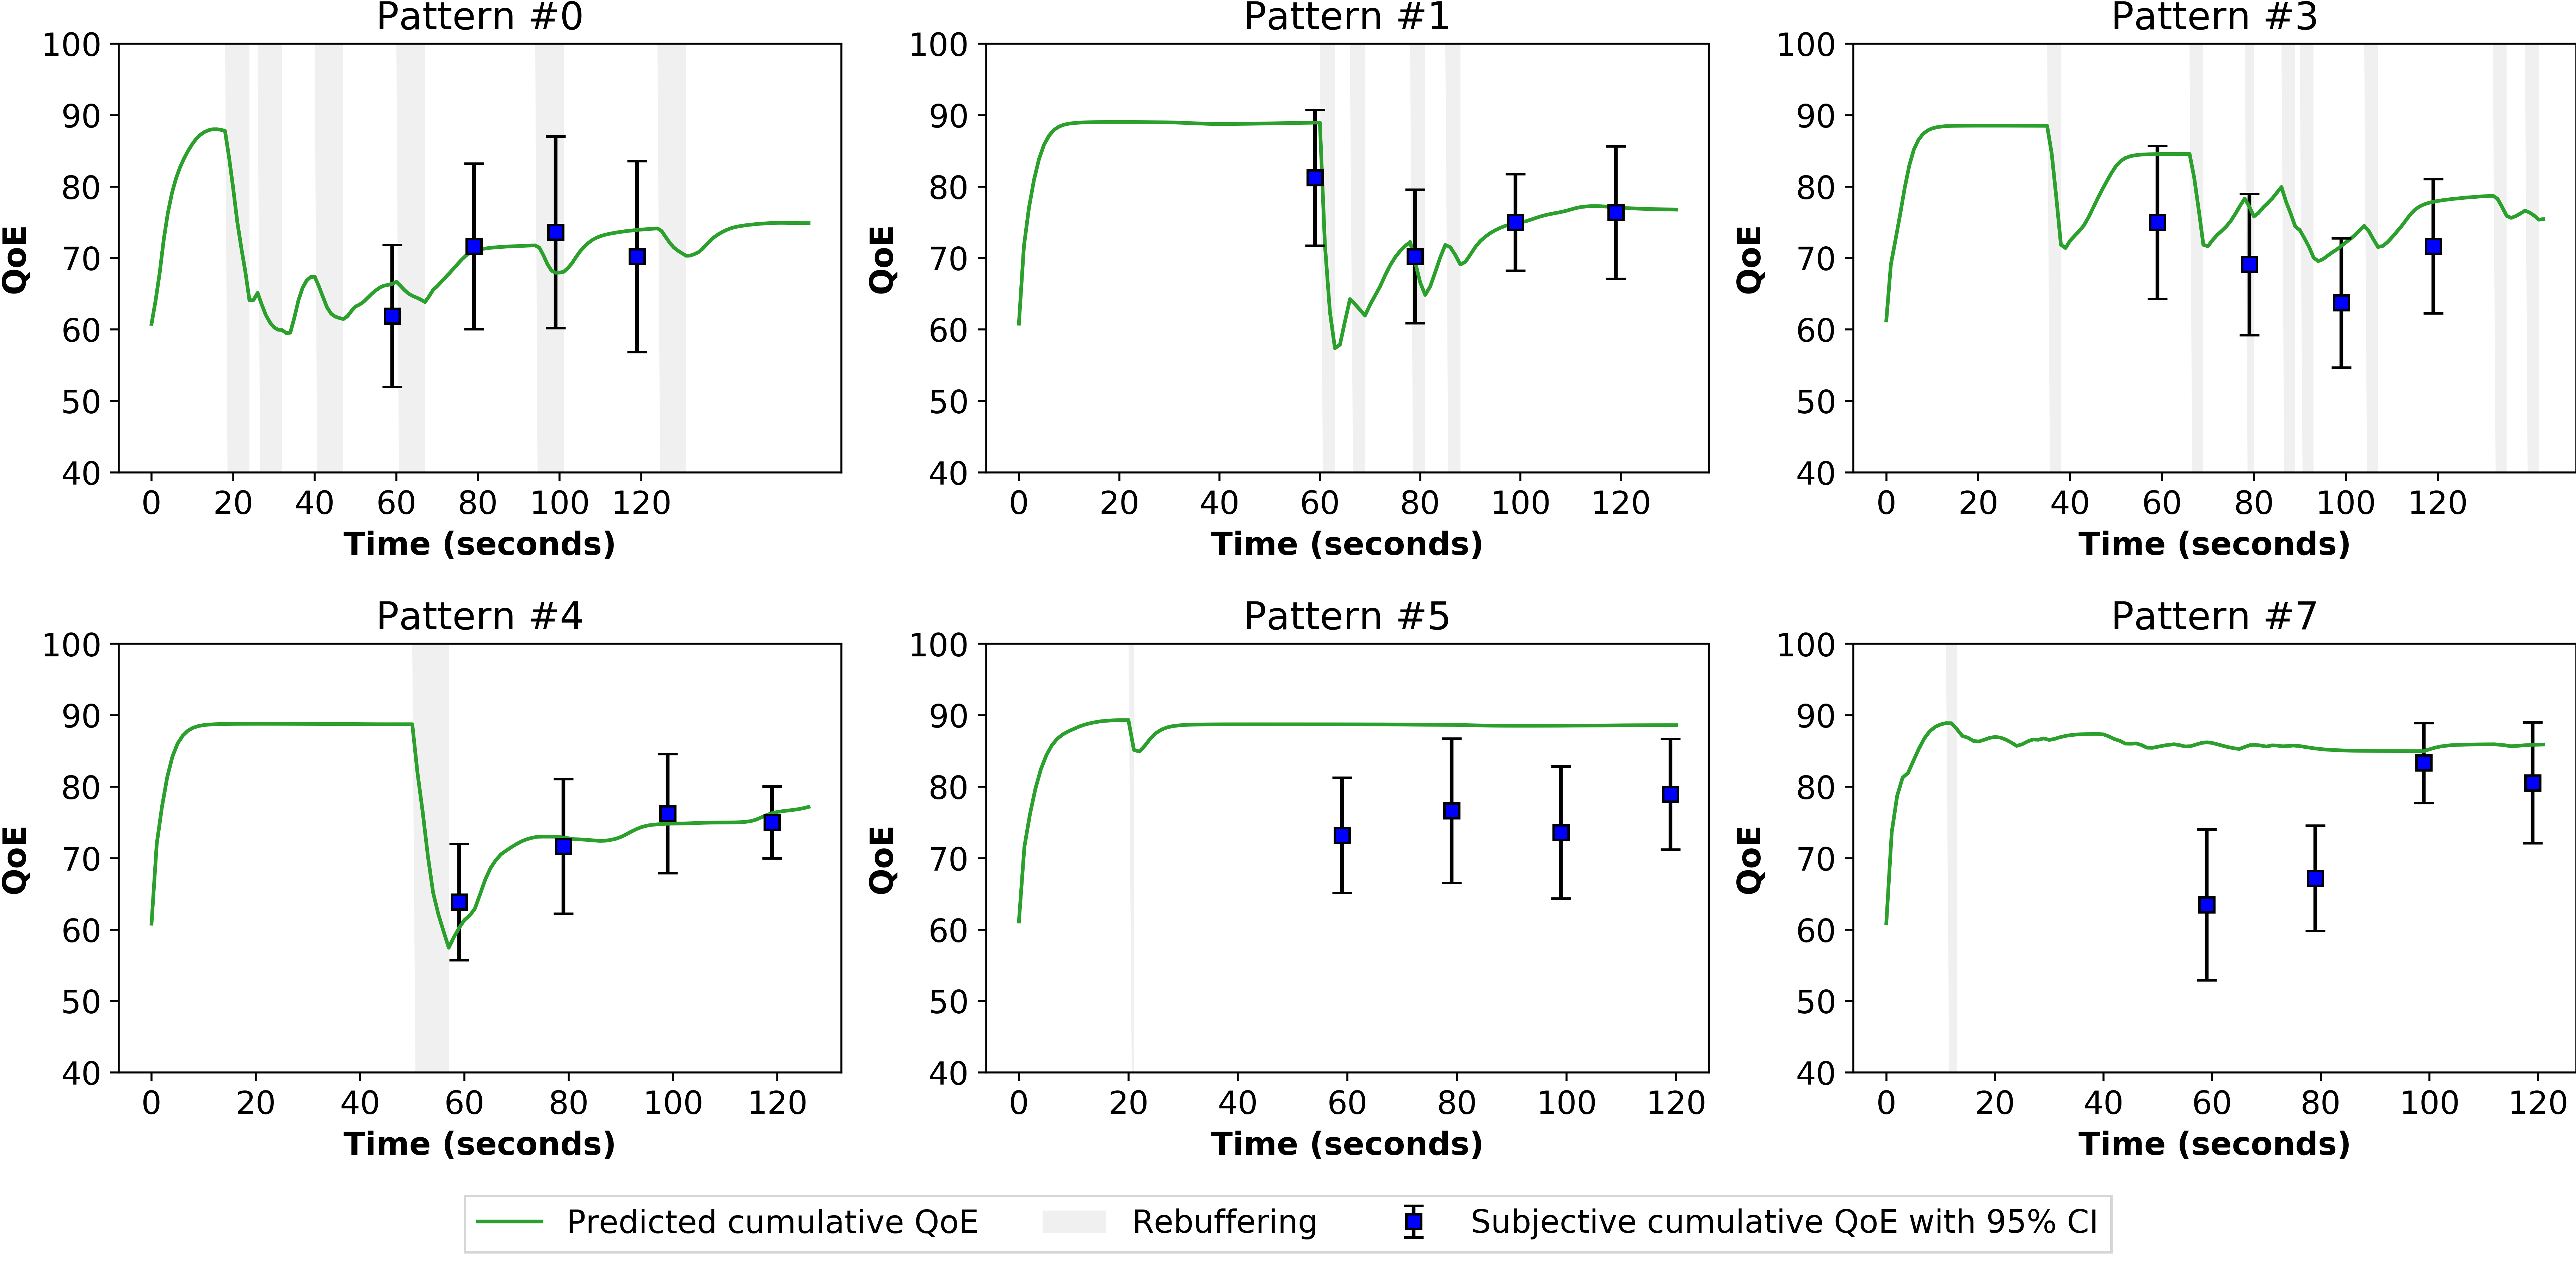
\includegraphics[width=\linewidth]{\FigsDir/cumulative_performance_experiment.png}
  \caption{Performance of our predicted cumulative QoE in comparison with the subjective cumulative QoE.}
  \label{fig:CumulativePerformanceExperiment}
\end{figure}

In this subsection, a subjective evaluation is conducted to assess the accuracy of the proposed model aligning with ground truth QoE scores provided by a number of subjects. The performance of QoE prediction using the proposed model is evaluated by relying on the following four measures: 1) PCC, 2) SROCC, 3) RMSE and 4) Outage Rate (OR) \cite{QoEModel_TimeVaryingSubjectiveQuality}. While PCC and SROCC quantify the correlation between predicted cumulative QoE and the subjective cumulative QoE, the closeness between predicted scores and the ground truth scores is numerically obtained by using RMSE and OR. In particular, OR measures the frequency of times when the prediction $p_{i}$ falls outside twice the confidence interval of subjective scores $s_{i}$, which is defined as the following equation:
\begin{equation}
    OR = \frac{1}{N}\sum^{N}_{i}{\mathbbm{1}(\left | p_{i} - s_{i} \right | > 2CI_{s_{i}} )}
\end{equation}
where $\mathbbm{1}$($\cdot$) is the indicator function

To conduct the subjective test, 6 distorted videos from the testing set of LFOVIA database (pattern \#0, \#1, \#3, \#4, \#5, \#7) were selected. We selected those videos because they have different contents, thus, the role of DoI in our model can be potentially assessed. Each distorted video was cropped into 4 small videos with starting timestamps of 00:00:00 and different length (60, 80, 100, and 120 seconds) using FFmpeg \cite{FFmpeg}. The purpose is to ask the subjects to provide subjective cumulative evaluations at the time points of 60, 80, 100, and 120 seconds of each distorted video. The correlations between subjective cumulative QoE and predicted cumulative QoE obtained from our model and reference model were assessed. The cropped videos were divided into 6 collections with different video content and displayed on a 15-inch screen with a resolution of 1920x1080 and a black background. Each video was rated by at least 18 subjects and there were totally 120 participants. Note that these subjects are different from those in "DoI" experiment in subsection 3.3. The Absolute Category Rating method was used in our experiment \cite{ITUT_P913}. The subjects give a rating score at the end of each cropped video with the score ranging from 1 (worst) to 5 (best) based on the perceived quality and video content, following the general principle of the ITU-T recommendation P.913 \cite{ITUT_P913}. The average of subjects scores, associated with 95\% confidence interval, for each cropped video, was utilized as the subjective cumulative QoE. These values were linearly rescaled so that the scores lay in the range [0, 100] and then compared with the predicted cumulative QoE.

Figure \ref{fig:PCC_CumulativeQoE_MOSQoE} illustrates the obtained correlation between the predicted cumulative QoE and subjective cumulative QoE. The comparison in QoE prediction performance between our model and reference model is tabulated in Table \ref{tbl:PerformanceExperiment}. Accordingly, we observe that the proposed model provides a competitive performance in terms of SROCC, RMSE and OR against the reference model. On the other hand, Fig. \ref{fig:CumulativePerformanceExperiment} shows a reasonable prediction performance of our model in comparison with subjective cumulative QoE at four discrete moments (at time points of 60, 80, 100, and 120 seconds) within a streaming session. In general, the proposed model performs extremely well when the high frequent and long duration rebuffering occur. It means that our model is capable of cumulatively capturing the effects of all the occurred unpleasant events on human perception. However, the model performance in pattern \#5 and \#7 are poorer, as compared to other patterns (\#0, \#1, \#4) even though they have only one short rebuffering event. This can be explained that in pattern \#5 and \#7, the users' perception seems to be significantly affected by the video content. In other words, the effect of DoI become dominant in their evaluation, which is not precisely captured by our model.


%/================================
\subsection{Computational Complexity}
  The computational complexity of the proposed model is determined by the computational complexity of forming the instantaneous QoE vector $Q_{t} = (q_{0}, q_{1},...,q_{t})$ predicted by the LSTM-QoE model.
  It is important to note that at the time instant $t$, the previous instantaneous QoE values $\{ q_{0}, q_{1},...,q_{t-1} \}$ have already been predicted and cached in the memory. Since the LSTM-QoE model takes up only a very small computational overhead to predict $q_{t}$ in order to form the vector $Q_{t}$, the cumulative QoE of each second $CQ_{t}$ can be predicted in real-time.
  To demonstrate this, we calculated the required computing time for training LSTM-QoE model and predicting the instantaneous QoE at the end of a session $q_{L}$. All the timing experiments were carried out on a 18.04 Ubuntu LTS Intel i7-8750H @ 2.20GHz and 16GB RAM system. The LSTM-QoE model took $620.740$ seconds to train and $0.4917$ milliseconds to predict $q_{L}$. Furthermore, the cumulative QoE $CQ_{L}$ prediction took $0.5103$ milliseconds. Thus the proposed model is suitable for real-time cumulative QoE prediction.


\subsection{Overall Evaluation}
\label{section:OverallEvaluation}
  In evaluation section, we assessed the performance of the model on a publicly available database and the subjective test. By doing this way, we can validate the predicted cumulative QoE in both quantitative and qualitative manners. Typically, the model can precisely provide cumulative QoE prediction in different scenarios. Therefore, the model promisingly provides an alternative and reliable approach in modeling QoE towards QoE based control and management.
  
  